\documentclass[10pt,aspectratio=32]{beamer}
\usepackage{sgp940}

\title{Box-Tidwell Transformation}
\subtitle{Realization with R language}
\vspace{1.5cm}
\author{Yi He \and ChengYu Huang \and JunJie Liu \\ \and JiaChen Tu \and DaiChen Yao }
\institute{United International College - STAT}
\date{\today}

\begin{document}
\AtBeginSection[]{\frame{\sectionpage}} %insert section title pages (new frames)

\begin{frame}
	\titlepage
\end{frame}

\begin{frame}
	\frametitle{Overview}
	\vspace{-0.7cm}
	\tableofcontents
\end{frame}

\section{Intro}
\subsection{Background}

\section{Procedure}
\subsection{Step Zero}
\subsection{Step One}
\subsection{Step Two}

%STEP BY STEP PROCEDURE
\begin{frame}
\frametitle{Step by Step Procedure}
\vspace{-0.3cm}

\textbf{Step Zero}

$$\begin{align}
&y = \beta_0 + \beta_1 w_1 + \dots + \beta_k w_k + \epsilon \label{eq:ordinary linear regression} \\
&w_j = f(x) =\left\{
\begin{aligned}
&x_j^{\alpha_j}  \alpha \neq 0 \\
&ln(x_j), \alpha = 0 \label{eq:ransformation of X}\\
\end{aligned}
\right.
\end{align}
$$
The method accommodates exponents on one or more of the regressor variables. $\alpha_1, \alpha_2, \dots,\alpha_k$
\end{frame}

\begin{frame}
	\frametitle{Step by Step Procedure (Continued)}
\textbf{Step One (Inital Model)}
\begin{itemize}
	\item Do a multiple linear regression: $$E(y_i) = \beta_0 + \beta_1 x_{1i} + \dots + \beta_k x_{ki}$$
	We denote the parameter estimates by $b_0, b_1, \dots, b_k$
	\item We can get: $z_j = x_j ln(x_j)$ which $x_j$ comes from the original model
	\item Do a regression of $y$ on $x_1, x_2, \dots, x_k, z_1, z_2, \dots, z_k$. Thus estimate $\gamma_1, \gamma_2, \dots, \gamma_k$, the coefficients of the $z$'s. Denote the estimates by $\hat{\gamma_1}, \hat{\gamma_2}, \dots, \hat{\gamma_k}$
	\item Estimate $\alpha_1, \alpha_2, \dots, \alpha_k$ by:
	$$\hat{\alpha_j} = \frac{\hat{\gamma_j}}{b_j} + 1 \ \ (j = 1, 2, \dots, k)\label{eq: estimates of alpha}$$
\end{itemize}
\end{frame}

\begin{frame}
 	\frametitle{Step by Step Procedure (Continued)}
 \textbf{Step Two (New Model and the Iteration)}

The results of equation \ref{eq: estimates of alpha} may be viewd as an updated estimate of $\alpha_j$. Often a one step computation is sufficient. Here is the procedure of the iteration model and the how to update the $\alpha$:

\begin{itemize}
	\item Use $w_1^* = x_1^{\hat{\alpha}}, w_2^* = x_2^{\hat{\alpha}} \dots, w_k^* = x_k^{\hat{\alpha_k}}$ to fit the model $$E(y_i) = \beta_0 + \beta_1 w_1^* + \dots + \beta w_k^*$$ with estimates $\hat{\beta_0}, \hat{\beta_1}, \dots, \hat{\beta_k}$
	\item Define $z_1^* = w_1^* ln(w_1^*), \ z_2 = w_2^* ln(w_2^*), \dots  ,z_k =w_k^* ln(w_k^*)$
	\item Fit a regression of $y$ on $w_1^*, w_2^*, \dots, w_k^*, z_1^*, z_2^*, \dots, z_k^*$ with a new coefficients of $z_1^*, z_2^*, \dots, z_k^*$ denoted by $\hat{\gamma_1}, \hat{\gamma_2}, \dots, \hat{\gamma_k}$
\end{itemize}

\end{frame}

\begin{frame}
 	\frametitle{Step by Step Procedure (Continued)}
 \textbf{Step Two (Update Term)}

 We compute the update $\hat{\alpha_j}$ with the formula:

 $$
 	\hat{\alpha_j} = (\frac{\hat{\gamma}_j}{\hat{\beta_j}} + 1) \times (\text{ Current Value of } \hat{\alpha_j})
 $$

We can get the new $\alpha$ for the new iteration, after $k$ times iterations $(|(\alpha_{k} - \alpha_{k-1}| \leq \epsilon$,$\epsilon$ is the tolrance value), we can stop the iteration and at that time, the $\alpha$ is what we need: the relative best fitting curve. In multiple regression it can also be a good use of this method, one more variable is to do a set of data loop.
\end{frame}



\section{R Code}
\subsection{get.beta.hat.R}
\subsection{boxtidwell.R}

\begin{frame}
 \frametitle{Code One}
 \vspace{-0.3cm}
	\begin{figure}[get.beta.hat]
		\centering
		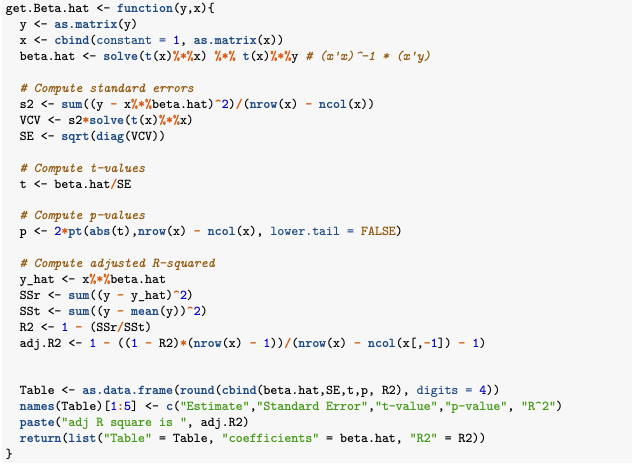
\includegraphics[width=0.9\textwidth]{get.png}
		\caption{get.beta.hat function}
	\end{figure}
\end{frame}

\begin{frame}
 \frametitle{Figure}
 \vspace{-0.3cm}
	\begin{figure}[get.beta.hat]
		\centering
		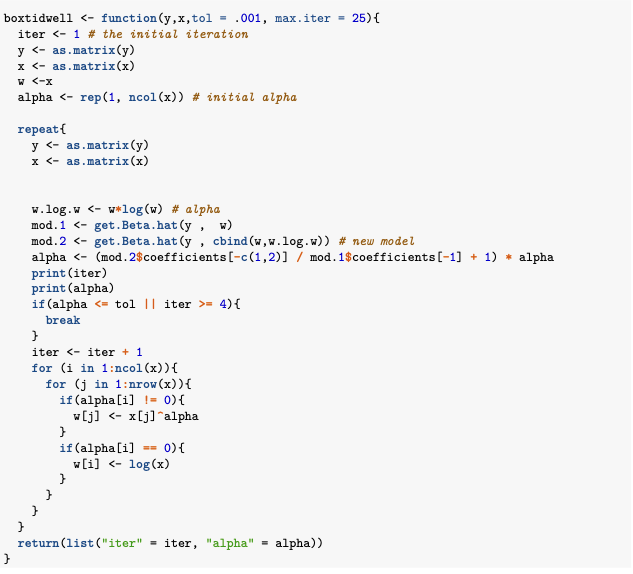
\includegraphics[width=0.75\textwidth]{box.png}
		\caption{get.beta.hat function}
	\end{figure}
\end{frame}

\section{Conclusion}

\begin{frame}
	\frametitle{References}
	\footnotesize{
		\begin{thebibliography}{99} % Beamer does not support BibTeX so references must be inserted manually as below
			\bibitem[Classical and Modern Regression with Applications (Second Edition)]{p293 - p 309} Raymond H.Myers (2005)
			\bibitem[car package - boxtiwell.R]{} Professor.John Fox (2010)
		\end{thebibliography}
	}
\end{frame}




\begin{frame}
 	\titlepage
\end{frame}

\end{document}
